\section{Mikołaj Majcherek}
\subsection{Przykładowe wyrażenie matematyczne}

\begin{math}
    \frac{1}{2\pi} \sum_{n=1}^{\infty} \left( \sqrt{\frac{2}{\pi}} \frac{\sin((2n-1)x)}{2n-1} - \frac{1}{2n-1} \right)
\end{math}

\subsection{Tabela}


\begin{table}[htbp]
    \centering
    \caption{Top 3 Mr. Olympia za czasów Ronniego Colemana}
    \begin{tabular}{|c|c|c|c|}
        \hline
        \textbf{Rok} & \textbf{Miejsce 1} & \textbf{Miejsce 2} & \textbf{Miejsce 3} \\
        \hline
        1998 & Ronnie Coleman & Flex Wheeler & Nasser El Sonbaty \\
        1999 & Ronnie Coleman & Flex Wheeler & Kevin Levrone \\
        2000 & Ronnie Coleman & Kevin Levrone & Flex Wheeler \\
        2001 & Ronnie Coleman & Jay Cutler & Kevin Levrone \\
        2002 & Ronnie Coleman & Kevin Levrone & Chris Cormier \\
        2003 & Ronnie Coleman & Kevin Levrone & Dexter Jackson \\
        2004 & Ronnie Coleman & Jay Cutler & Gustavo Badell \\
        2005 & Ronnie Coleman & Jay Cutler & Dexter Jackson \\
        \hline
    \end{tabular}
    \label{tab:top3_mrolympia}
\end{table}


\subsection{Lista Numerowana}

\begin{enumerate}
    \item 8-krotne zwyciestwo w Mr. Olympia.
    \item Rekordowa liczba zwyciestw w zawodach IFBB.
    \item Nieprawdopodobne osiagniecia silowe.
\end{enumerate}

\subsection{Lista Nieumerowana}

\begin{itemize}
    \item Dyscyplina i determinacja.
    \item Upór i pokonywanie przeciwności.
    \item Charyzma i pozytywne podejście.
\end{itemize}

\subsection{Tekst}

Ronnie Coleman, urodzony 13 maja 1964 roku w Monroe, Luizjana, USA, to byly profesjonalny kulturysta, powszechnie uwazany za jedna z najbardziej utalentowanych postaci w historii tego sportu. Osiagnal prestizowy tytul Mr. Olympia az osiem razy z rzedu w latach 1998-2005, co potwierdza jego dominacje na swiatowej scenie kulturystycznej.

Poza sukcesami w kulturystyce, Coleman byl rowniez funkcjonariuszem policji, co dodaje nowego wymiaru do jego wielowarstwowej osobowosci. Jego niezwykla sila fizyczna i imponujaca sylwetka uczynily go ikona w swiecie kulturystyki. Znany ze swojego zdyscyplinowanego i zdeterminowanego podejscia do treningu, Coleman nadal inspiruje entuzjastów fitnessu na calym swiecie.


\subsection{Zdjecie}

\begin{figure}[htbp]
    \centering
    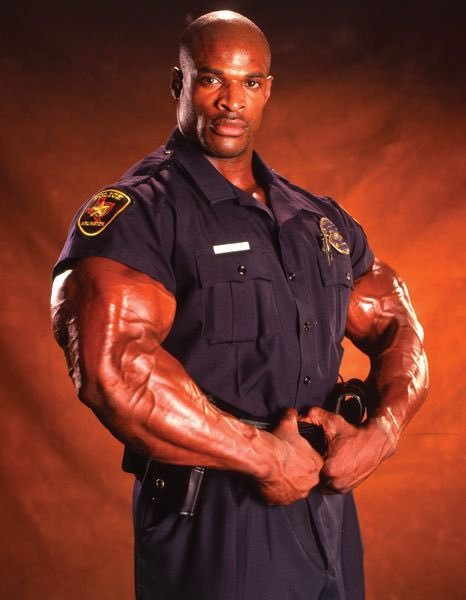
\includegraphics[width=0.5\textwidth]{pictures/policjant.jpg}
    \caption{Ronnie Coleman był policjantem.}
    \label{fig:zdjecie}
\end{figure}
